
Dendrimers of the SPL family are a challenging test case for pyPolyBuilder.
Among the examples considered in this tutorial, this is the most complex case for the dendrimer module.
Its structure for a generation 1 dendrimer is illustrated in Figure \ref{fig:SPL7013G1}.

\begin{figure}
    \centering
    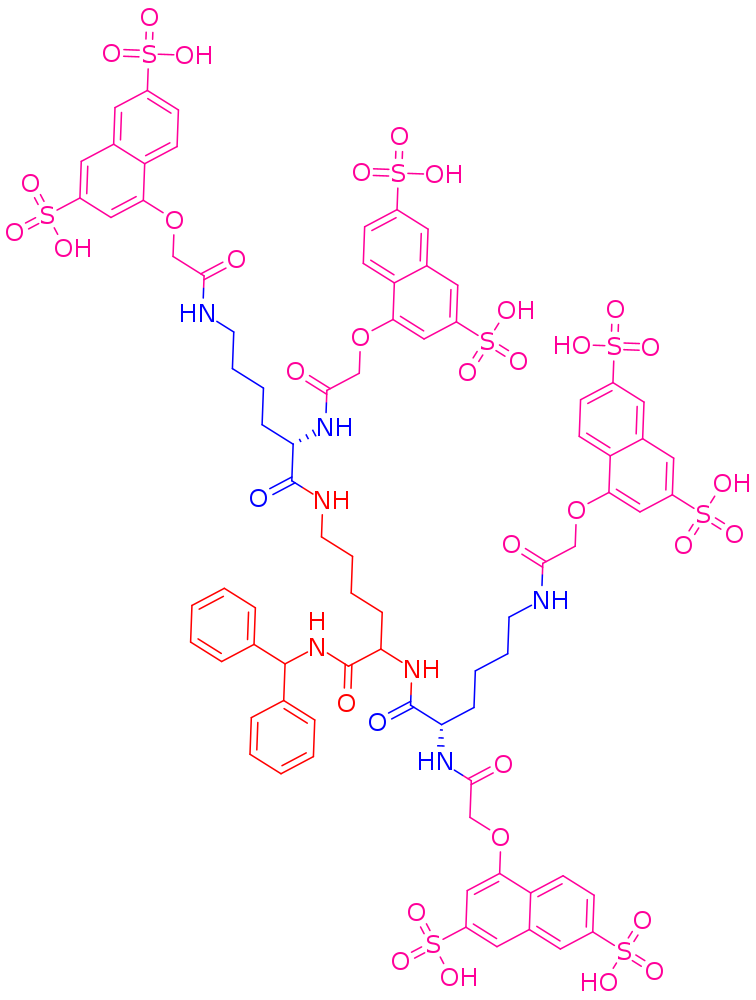
\includegraphics[width=0.5\textwidth]{SPL7013/SPL7013G1.png}
    \caption{SPL G1 dendrimer.
            The benzhydrylamine core is illustrated in red, the intermediaries lysine is in blue and the terminals naphthalene disulfonate acid is in pink.
             }
    \label{fig:SPL7013G1}
\end{figure}

The division for the SPL BBs was made as the colors suggest in Figure \ref{fig:SPL7013G1}.
The benzhydrylamine bonded to a lysine is chosen to be the core, a lysine molecule alone is the intermediary block and the napthtalene disulfonate is the terminal block.
The BBs themselves are illustrated in Figure \ref{fig:SPL7013BB}.

\begin{figure}
    \centering
    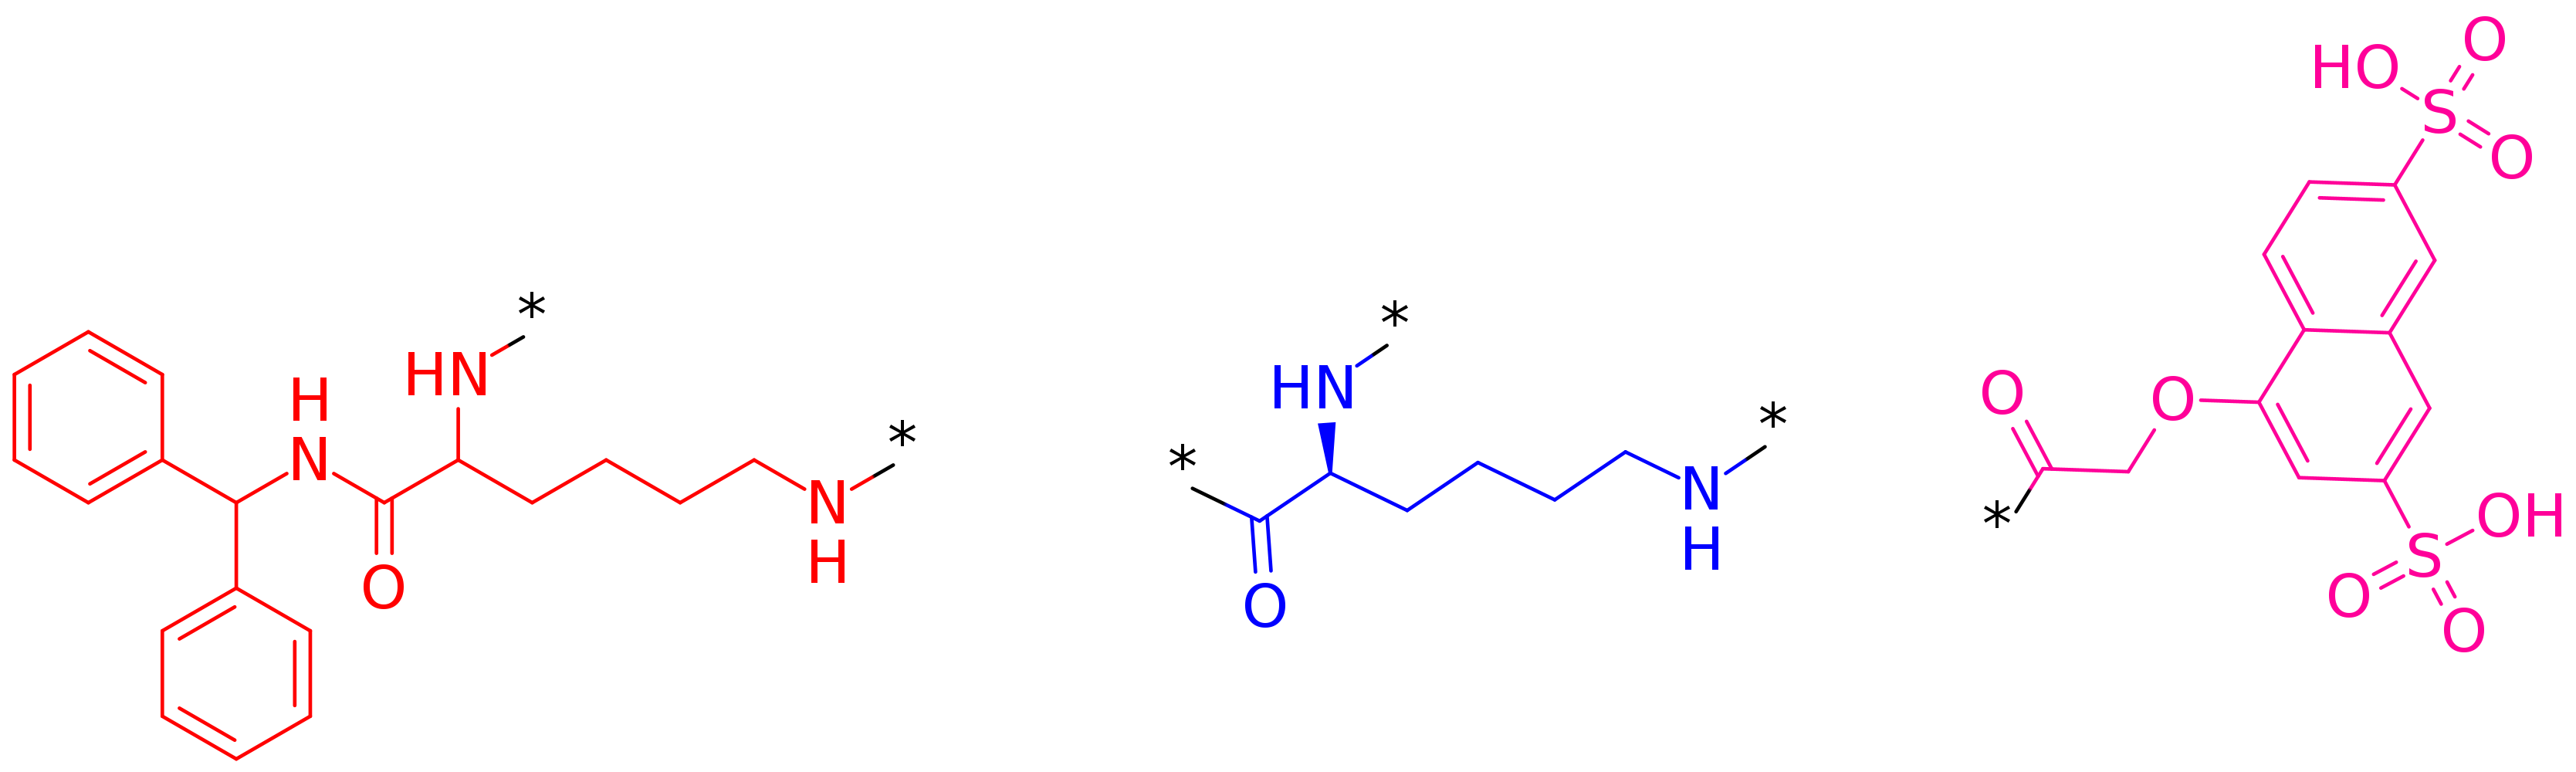
\includegraphics[width=\textwidth]{SPL7013/SPL7013BBs.png}
    \caption{SPL7013 dendrimer BBs.
             The colors were chosen to match the ones illustrated in Figure \ref{fig:SPL7013G1}.}
    \label{fig:SPL7013BB}
\end{figure}

MTFs for those BBs are available in the tutorial directory in pyPolyBuilder root, which structure is illustrated below:
\begin{lstlisting}
<path/to/pypolybuilder>/demo/gromacs_format/dendrimer/SPL7013
\end{lstlisting}
\dirtree{%
.1 SPL7013.
.2 core\_BHA.itp.
.2 inter\_LYS.itp.
.2 ter\_NDSA.itp.
.2 list\_param.itp.
.2 run.
.3 SPL7013.sh.
.3 SPL7013.top.
.3 mdp.
}

The MTFs are named according to its block and molecule name.
The core\_BHA.itp is the benzhydrylamine core BB, inter\_LYS.itp the lysine intermediary block and the ter\_NDSA.itp is the naphtalene disulfonate acid terminal block.

The command line below can be used to build a generation 1 SPL dendrimer (Figure \ref{fig:SPL7013G1}):

\begin{lstlisting}
python3 ../../../../__main__.py \
--core=core_BDA.itp \
--inter=inter_LYS.itp \
--ter=ter_NDSA.itp \
--params=list_param.itp \
--ngen=1 \
--name=SPL \
--output=SPL.itp \
--gro=SPL.gro \
--nsteps=5000 \
--nskipLJ=100 \
--gromacs \
--stepLength=0.0001 \
--forcefield=../../../../gromos2016h66.ff \
--dendrimer
\end{lstlisting}

Some of the used option were already used in previous tutorials and explained in Section \ref{sec:CommandLine}.
\texttt{--core}, \texttt{--inter} and \texttt{--ter} are used to select the dendrimer BBs and \texttt{--ngen} to select its generation number.
\texttt{--name}, \texttt{--output} and \texttt{--gro} are used to name the topology, the MTF itself and the geometry coordinates file, respectively.
\texttt{--gromacs} is used to define the format of the output files, in this case, in the gromacs format.
Even though \texttt{--gromacs} is the default, \texttt{--gromos} is also available.
\texttt{--nsteps} set how many steps will be made in geometry optimization step.
PyPolyBuilder stops the iteration if the energy converges or if the \texttt{nstep} is reached.
Before doing a local minimization to carry the geometry to a local minimum, pyPolyBuilder carry out a genetic algorithm (GA) optimization only for the torsional dihedrals in order to set a initial quasi-optimum geometry that will be optimized in the local minimization step.
Due to the stochastic nature of GA, in very complex geometries it is possible that some atoms are very close at the end of the GA optimization.
To avoid these bad interactions, \texttt{--nSkipLJ} set how many steps of the geometry optimization will be carried out without evaluating Lennard-Jones (LJ) interactions.
Turning LJ interactions off for the first few steps allows the structure to relax only using bonded potentials avoiding bad contacts.
\texttt{--stepLength} set the size of the minimization step.
Also for complex systems, it is possible that the output of GA is far from optimum.
So \texttt{--stepLength} can be used to allow a slow minimization in order to avoid overlaps.
pyPolyBuilder has default values for bonded and non-bonded parameters.
Because of that, the generated structure may not actually be at the minimum of the desired force field.
Using the \texttt{--forceField} flag, one can pass to pyPolyBuilder the location of a force field (FF) in gromacs format to be used in the geometry optimization. 
It may be possible in some cases that the built-in FF is not good enough.

SPL is, for instance, a real challenge due to its very complex structure.
In this tutorial, 2016H66 FF was used to optimize its geometry, the built-in FF lead to an unphysical geometry in which some of the bonds were too long and others were too short (it can be tested by removing the \texttt{--forcefield} flag from the previous command-line).
Besides, the obtained structure may be equally problematic if the \texttt{--nsteps} keyword is not used.

This is a really specific and singular dendrimer.
The fact that the pyPolyBuilder is able to build this structure proofs its versatility and robustness.

After pyPolyBuilder finish the optimization step, one can use any visualization software (such as vmd or pymol) to check the output geometry. 
Note that the coordinates are generated considering a dendrimer without any partial charge in vaccum.
Hence, the obtained conformation is probably not fully realistic.
However, if one wants to test the topology of this purely academic case, the run directory has some scripts to run a short molecular dynamics in order to equilibrate the molecule in water using gromacs.
These scripts were developed for a specific architecture and should be adapted by the user.

\begin{figure}
    \centering
    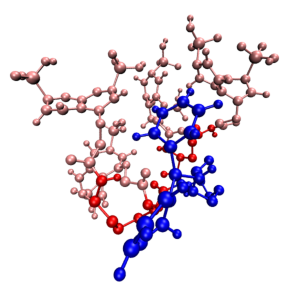
\includegraphics[width=0.5\textwidth]{SPL7013/SPL1.pdf}
    \caption{SPL G1 dendrimer built by pyPolyBuilder.
             The colors were chosen to match Figure \ref{fig:SPL7013G1}.}
    \label{fig:SPL7013PPB}
\end{figure}

Using the available scripts in the run directory to run a small equilibration after solvation and energy minimization in gromacs package, one can see the structure of SPL G1 dendrimer in Figure \ref{fig:SPL7013SOL}.

\begin{figure}
    \centering
    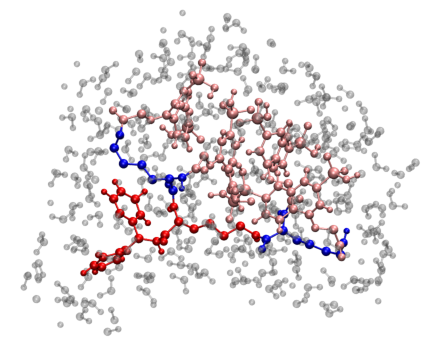
\includegraphics[width=0.5\textwidth]{SPL7013/SPLSOL.pdf}
    \caption{SPL G1 dendrimer equilibrated in water.
             The colors were chosen to match Figure \ref{fig:SPL7013G1}.
             Water molecules are illustrated as the translucent gray molecules.}
    \label{fig:SPL7013SOL}
\end{figure}

